\subsubsection{Gl{\"u}ck} \label{glueck-4}



\todo[inline,color=green!40]{Verantwortlich: Minas\\
- RfP}




Um das Gl{\"u}ck-Szenario in einer VR-Umgebung zu verwirklichen, wurden sich f{\"u}r HDR-Panorama-Bilder entschieden, die in Unreal eine Umgebung bilden sollen. 
Der Grund weswegen die Bilder HDR und Panorama sein m{\"u}ssen, werden im Laufe dieses Kapitels erkl{\"a}rt. 
Au{\ss}erdem wird eine Audio-Datei im Hintergrund abgespielt und ein Text eingeblendet, welches thematisch zum Bild passt. 
Die Grundidee stammt vom ersten Prototypen (Kapitel 7.3.1), welches nicht in einer VR-Umgebung gel{\"o}st wurde. 
In Kapitel 7.3.1 wurde zudem erkl{\"a}rt, weshalb und welche Audio-Datei im Hintergrund abgespielt wird, weshalb die Texte eingeblendet werden und was sich unter Gl{\"u}ck verstehen l{\"a}sst. \\

Insgesamt besteht das Gl{\"u}ck-Szenario aus acht HDR-Panorama-Bilder f{\"u}r das Hauptszenario und ein HDR-Panorama-Bild f{\"u}r das Warm-Up-Szenario. 
Abbildung \ref{fig-glueck4} zeigt alle Bilder die genutzt werden und deren Texte (falls vorhanden). \\

\begin{figure}[H] \centering
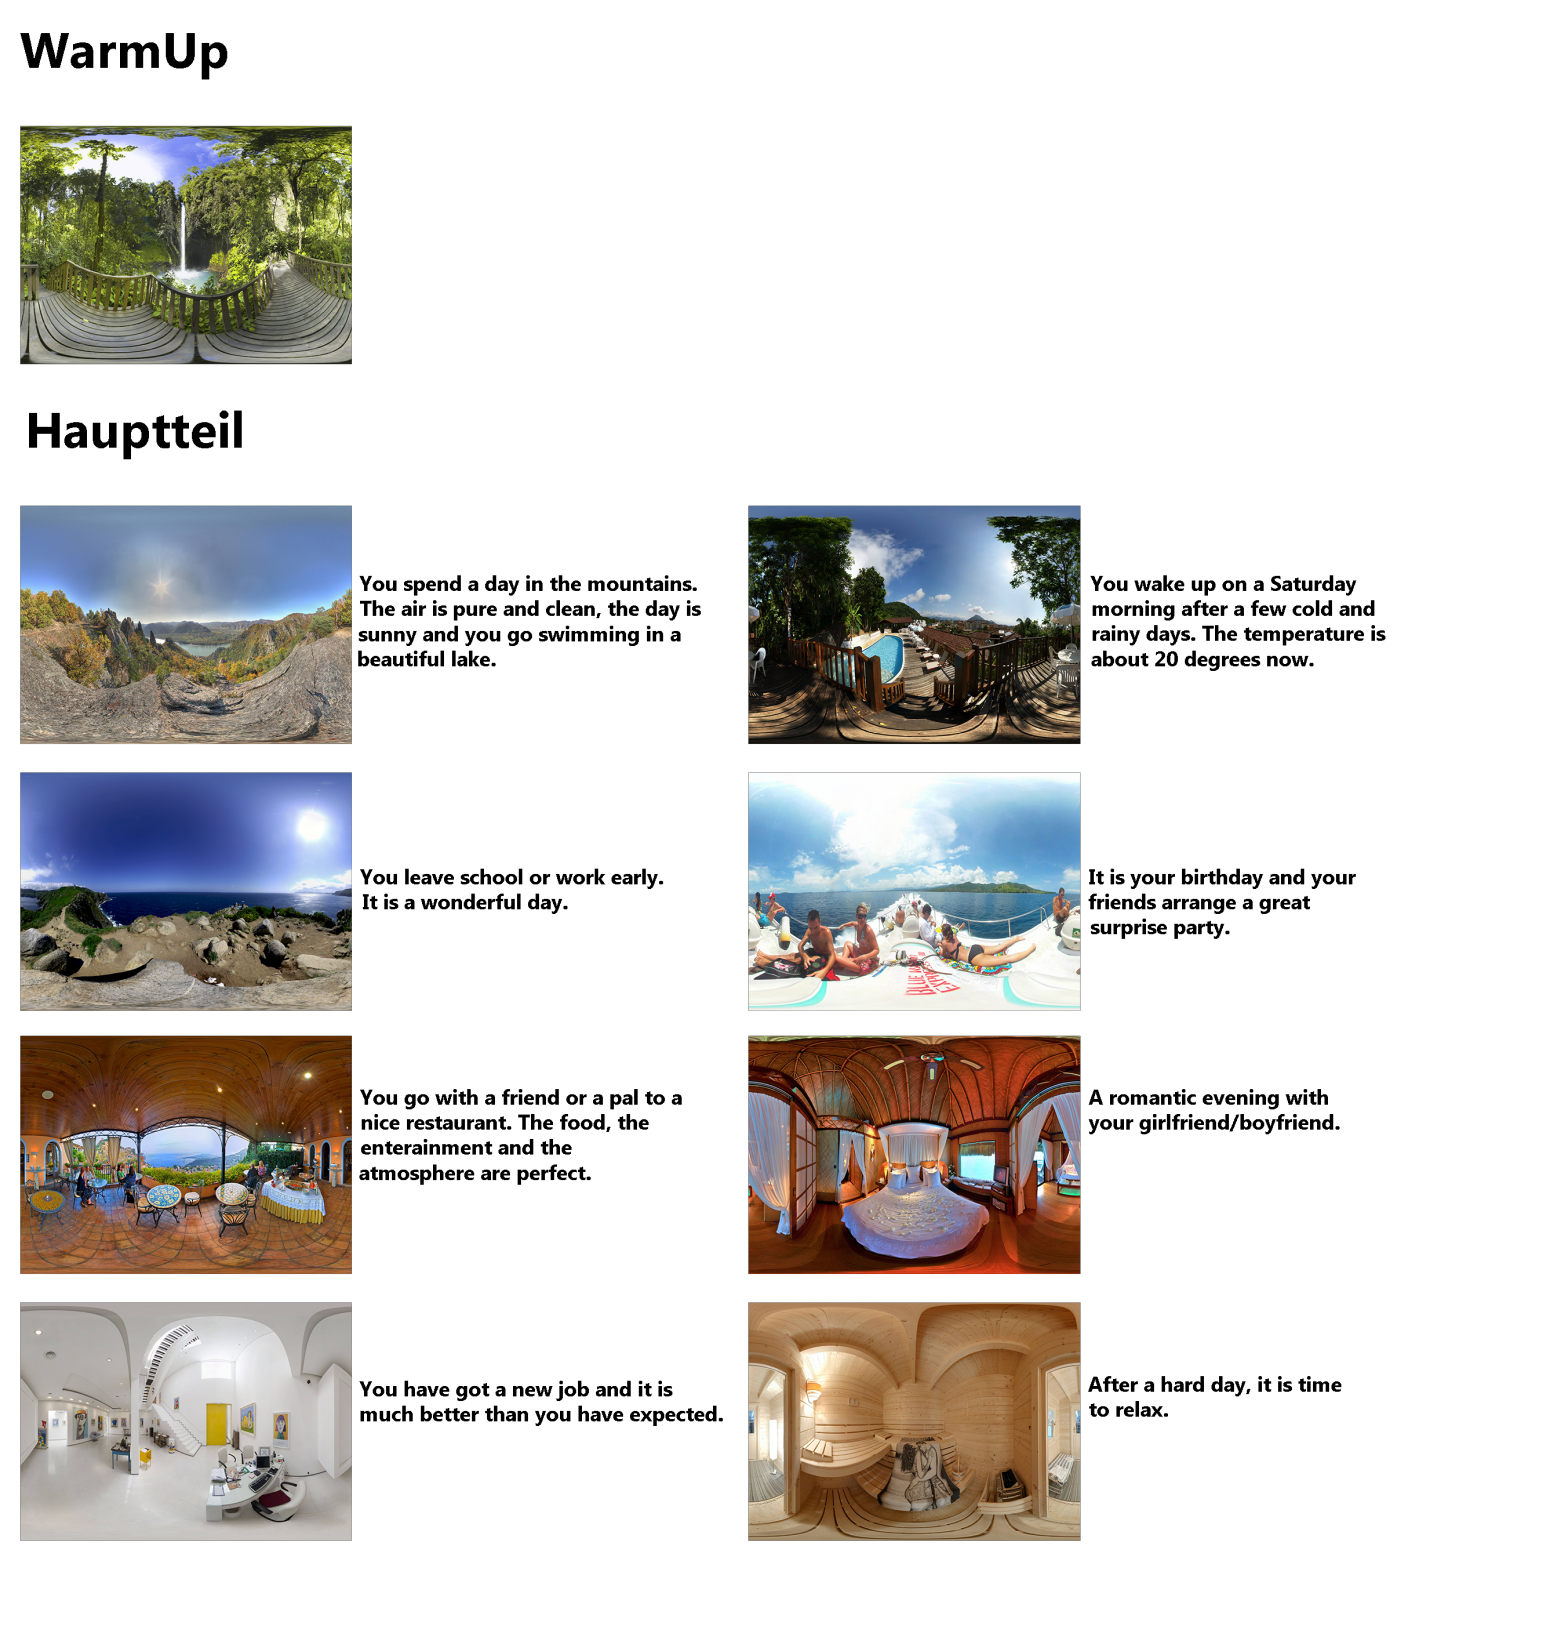
\includegraphics[width=15cm]{Images/gluck4.png} 
\vspace{-0.3cm} 
\caption[Im Gl{\"u}ck-Szenario verwendete Bilder und deren Texte]{Im Gl{\"u}ck-Szenario verwendete Bilder und deren Texte\cite{sun360}.}
\label{fig-glueck4} 
\end{figure}


Die Bilder lassen sich jedoch nicht ohne weiteres in Unreal einbinden. 
Um dies zu realisieren wurde sich f{\"u}r eine CubeMap in DDS-Format entschieden. 
Hierf{\"u}r m{\"u}ssen die Bilder zun{\"a}chst durch verschiedene Tools (Blender, Photoshop) bearbeitet werden und dann mit bestimmten Konfigurationen in Unreal eingebunden werden. \\

\begin{figure}[H] \centering
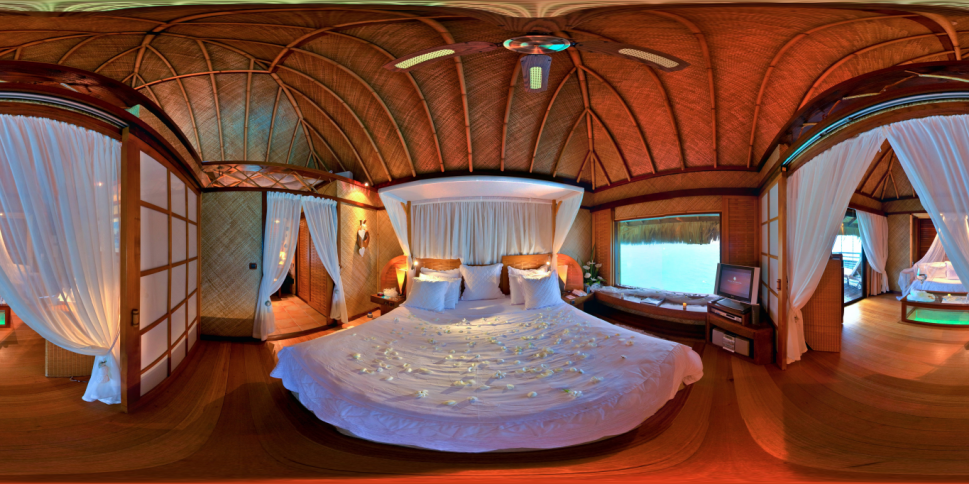
\includegraphics[width=\textwidth]{Images/hdr-panorama.png} 
\caption{Ein im Projekt verwendetes HDR-Panorama-Bild.}
\label{fig-hdr} 
\end{figure}


Anhand Abbildung \ref{fig-hdr} wird die Bearbeitung der Bilder erkl{\"a}rt. 
Nach Auswahl eines Panorma-HDR-Bildes, wird dieses in Blender bearbeitet. 
Blender wird ben{\"o}tigt, um aus dem gesamten Bild, sechs Einzelbilder mit der ben{\"o}tigten Rotation zu erzeugen. 
Das ist der erste Schritt um sp{\"a}ter eine CubeMap zu erzeugen. 
Im Internet existiert bereits eine Blender-File mit den ben{\"o}tigten Konfigurationen\cite{facerig19}, um an diese Einzelbilder zu gelangen. 
Diese besteht aus einer Kamera, welches um das importierte Bild rotiert und dieses zurecht schneidet. 
Handelt es sich um kein Panorama Bild, werden die sechs Bilder falsch geschnitten und k{\"o}nnen dadurch die Kriterien einer CubeMap nicht erf{\"u}llen. \\

\begin{figure}[H] \centering
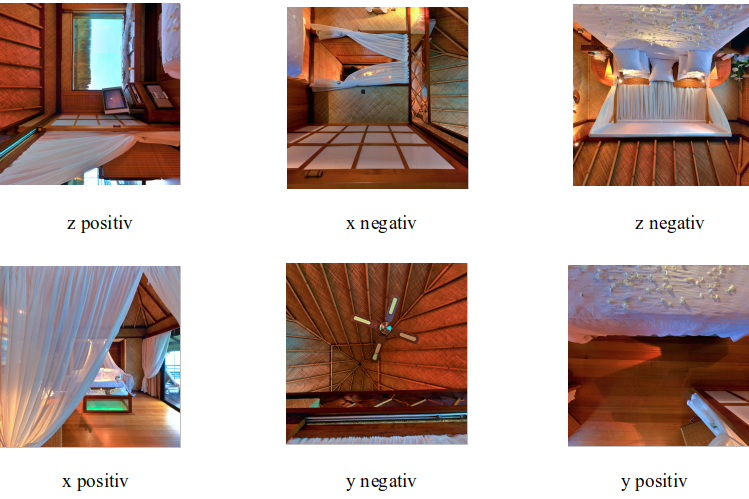
\includegraphics[width=\textwidth]{Images/blender-bilder.png} 
\caption{Ausgabe der Blender-File und deren Rotation.}
\label{fig-blender-bilder} 
\end{figure}


Um eine CubeMap in Unreal einzubinden, wird jedoch nur ein Bild im DDS-Format ben{\"o}tigt und nicht sechs Einzelbilder. 
DDS steht f{\"u}r Direct Draw Surface und ist ein entwickeltes Format von Microsoft. 
Dieses Format wird haupts{\"a}chlich f{\"u}r die Speicherung von CubeMaps und Texturen verwendet und erh{\"o}ht die Geschwindigkeiten in Spielen ohne Verlust von Details\cite{dateiendungen19}.
Nvidia bietet ein Plugin f{\"u}r einige Adobe Photoshop Versionen und GIMP, um CubeMaps in DDS-Format abzuspeichern.
Der n{\"a}chste Schritt eine CubeMap zu erstellen, wurde mit Adobe Photoshop CS2 und dem Nvidia Texture- Plugin realisiert. 
Hierf{\"u}r m{\"u}ssen die Bilder in Abbildung \ref{fig-blender-bilder} in richtiger Reihenfolge aneinander gereiht werden. 
Dies geschieht in Adobe Photoshop. 
Die ben{\"o}tigte Reihenfolge wird in Abbildung \ref{fig-rotation} gezeigt. \\

\begin{figure}[H] \centering
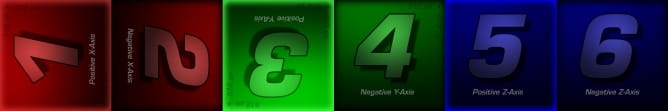
\includegraphics[width=\textwidth]{Images/rotation.png} 
\caption[Rotation und Reihenfolge f{\"u}r eine CubeMap]{Rotation und Reihenfolge f{\"u}r eine CubeMap\cite{franczak19}.}
\label{fig-rotation} 
\end{figure}


Somit ergibt sich f{\"u}r die Bearbeitung der Abbildung \ref{fig-blender-bilder}, Abbildung \ref{fig-blender-bilder2}. \\

\begin{figure}[H] \centering
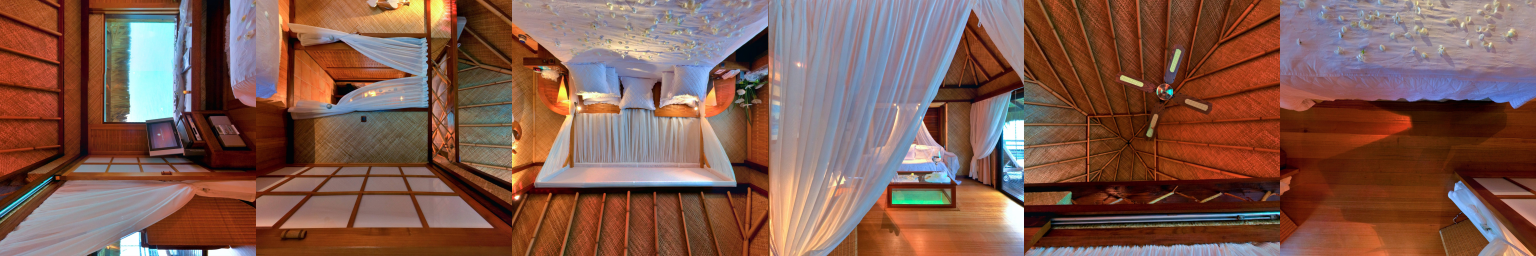
\includegraphics[width=\textwidth]{Images/blender-bilder2.png} 
\caption{Rotation und Reihenfolge f{\"u}r die CubeMap der Abbildung \ref{fig-blender-bilder}.}
\label{fig-blender-bilder2} 
\end{figure}


Nach einer aneinander Reihung der einzelnen Bilder, l{\"a}sst sich das dadurch entstandene Bild mit Hilfe des Nvidia Plugins in eine DDS-File exportieren. 
Somit wird die gew{\"u}nschte Cubemap generiert.
Abbildung \ref{fig-cubemap} zeigt die aufgeklappte Form einer CubeMap.
Jetzt kann die DDS-File in Unreal importiert bzw. konfiguriert werden. \\

\begin{figure}[H] \centering
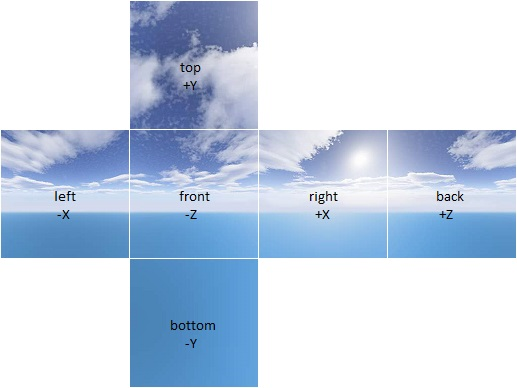
\includegraphics[width=\textwidth]{Images/cubemap.png} 
\caption[Aufgeklappte CubeMap]{Aufgeklappte CubeMap\cite{belanec19}.}
\label{fig-cubemap} 
\end{figure}


Sobald die DDS-File im Unreal-Projekt importiert wurde, muss an der DDS-File selbst Einstellungen vorgenommen werden. 
Abbildung \ref{fig-einstellungen} beinhaltet die optimalen Einstellungen. \\

\begin{figure}[H] \centering
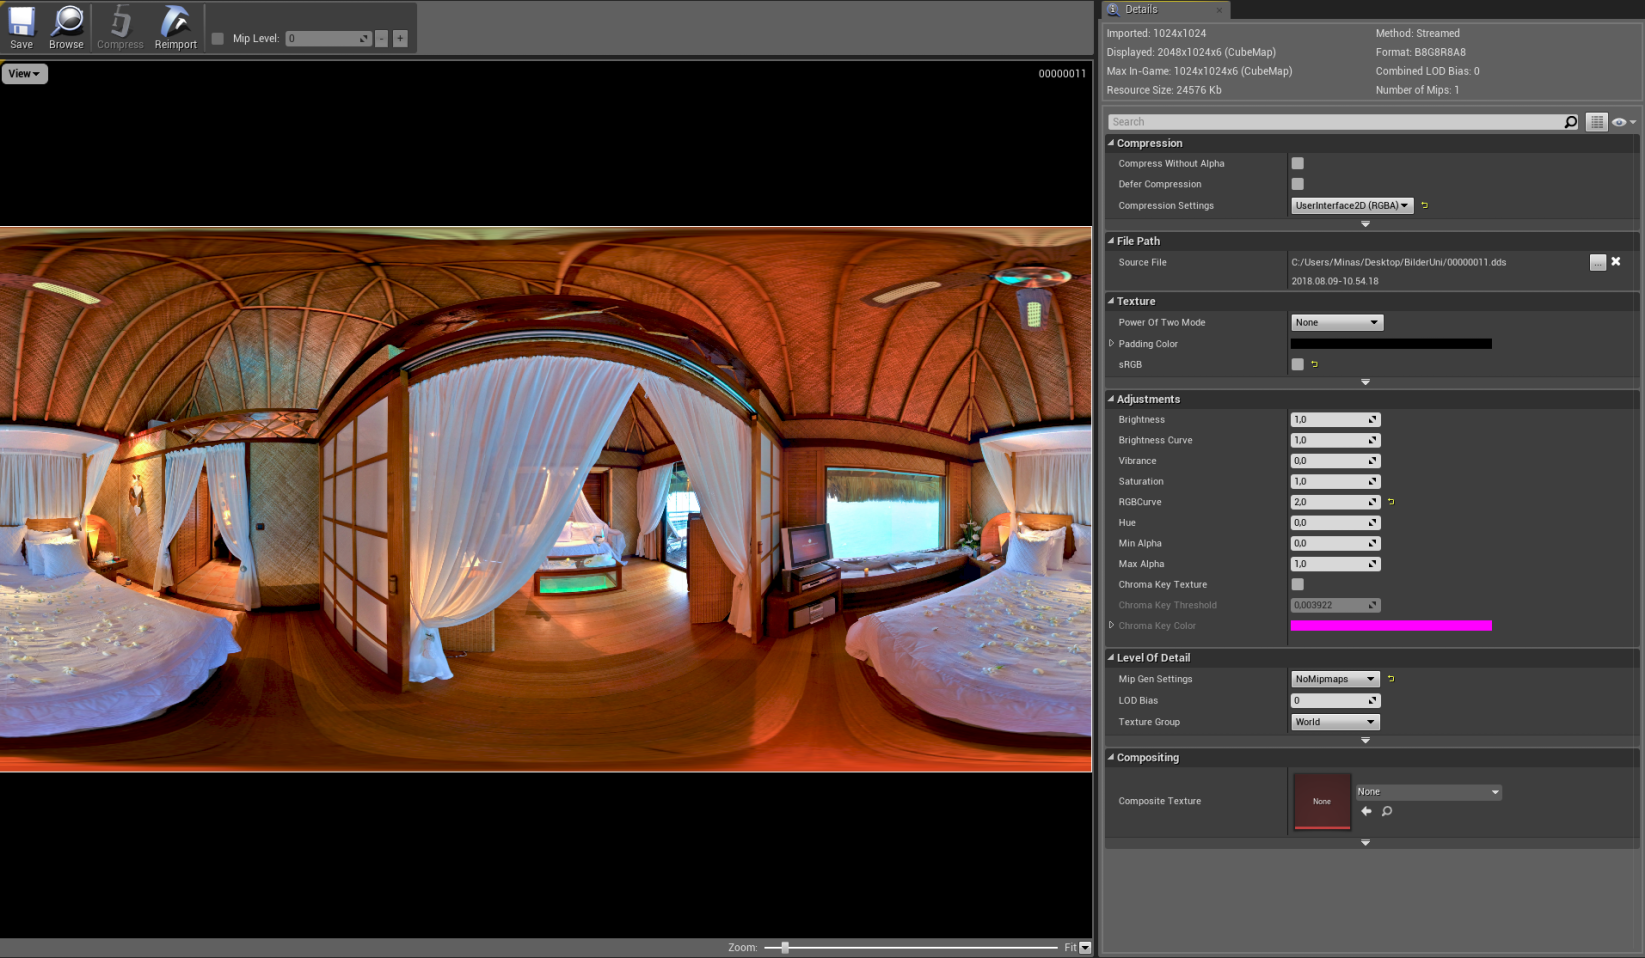
\includegraphics[width=\textwidth]{Images/einstellungen.png} 
\caption{Optimale Einstellungen des Bildes in Unreal.}
\label{fig-einstellungen} 
\end{figure}


Diese Einstellungen lassen sich f{\"u}r alle Bilder {\"u}bernehmen. 
Lediglich die Einstellung RGBCurve unter ``Adjustments'' muss von Bild zu Bild variiert werden. 
Desto h{\"o}her der eingetragene Wert, umso kr{\"a}ftiger werden die Farben des Bildes. 
Wird der Standardwert von ``1,0'' gelassen, wirkt das Bild sehr blass und ist damit nicht anschaulich. 
Hier spielt auch die Qualit{\"a}t des Bildes eine gro{\ss}e Rolle. 
Am Anfang des Kapitels wurde HDR erw{\"a}hnt. 
HDR steht f{\"u}r High Dynamic Range und erm{\"o}glicht ein gr{\"o}{\ss}eren Helligkeitsbreich als SDR (Standard Dynamic Range). 
Es l{\"a}sst das Bild realistischer wirken, ohne Farbt{\"o}ne im dunklen oder hellen Bereichen zu vernachl{\"a}ssigen\cite{eizo19}.
Abbildung \ref{fig-sdr-hdr} zeigt den Qualit{\"a}tsunterschied zwischen SDR und HDR.
Es ist von Vorteil ein solches Format zu verwenden, um eine gute VR-Umgebung zu realisieren. \\

\begin{figure}[H] \centering
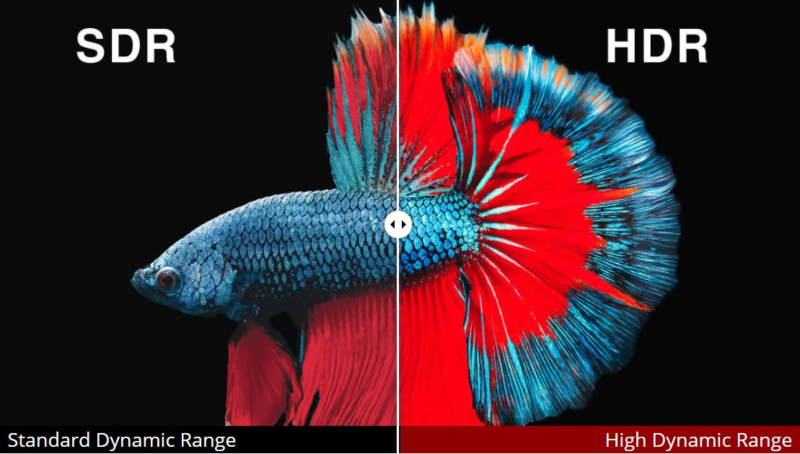
\includegraphics[width=8cm]{Images/sdr.png} 
\caption[SDR vs. HDR]{SDR vs. HDR\cite{finch19}.}
\label{fig-sdr-hdr} 
\end{figure}


Nach dem das Bild in Unreal fertig konfiguriert wurde, muss eine ``Blueprint Class'' angelegt werden. 
Diese wird in diesem Beispiel ``SkySphere-BP'' genannt. 
In diesem Blueprint wird eine Variable angelegt mit dem Namen ``SkyMaterial''. Au{\ss}erdem sollte das Construction Script wie in Abbildung \ref{fig-skysphere} aufgebaut sein. \\

\begin{figure}[H] \centering
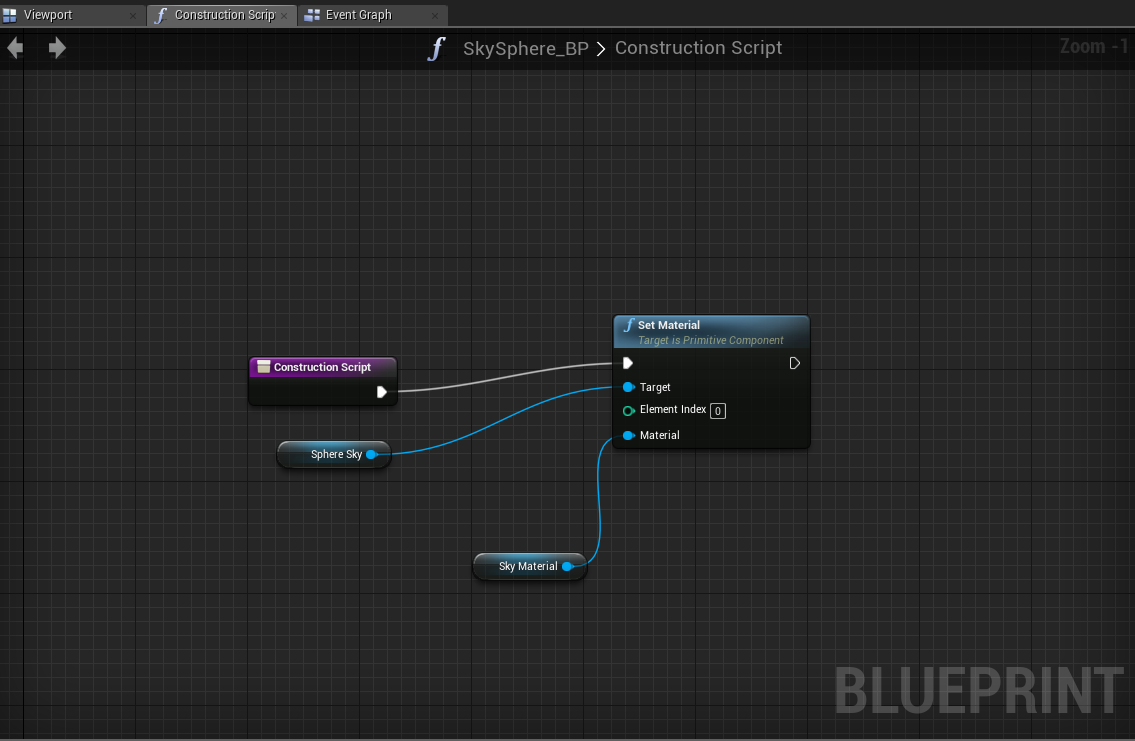
\includegraphics[width=8cm]{Images/skysphere.png} 
\caption{SkySphere-BP Construction Script.}
\label{fig-skysphere} 
\end{figure}


Mit diesem Construction Script lassen sich CubeMaps in die SkySphere importieren und bei Bedarf auch austauschen. \\

Nun muss ein Material f{\"u}r die SkySphere erstellt werden. Abbildung \ref{fig-konfiguration} zeigt wie diese Konfiguriert werden sollte. \\

\begin{figure}[H] \centering
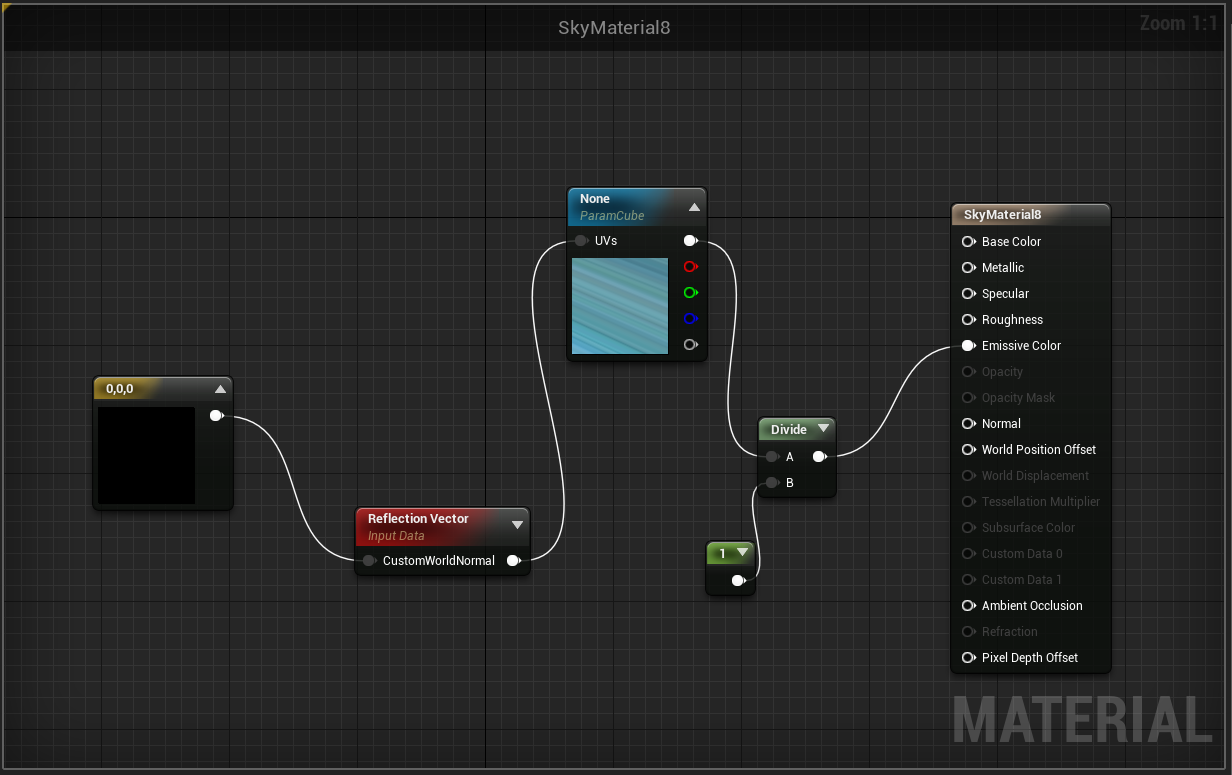
\includegraphics[width=8cm]{Images/konfiguration.png} 
\caption{Konfigurationen von Material.}
\label{fig-konfiguration} 
\end{figure}


Im Knoten ``ParamCube'' muss die Textur ausgesucht werden. 
In diesem Fall handelt es sich um die erstellte CubeMap. 
Als letztes muss das erzeugte Material der SkySphere zugewiesen werden. 
Nun l{\"a}sst sich die Umgebung in Unreal anzeigen.
Der Text im Bild l{\"a}sst sich mit einem Blueprint-Pawn erzeugen. 
Die Position des Textes wird manuell vorgenommen, in dem der Text im Bild verschoben wird. 
Damit der {\"u}bergang zwischen den Bildern angenehm f{\"u}r die Probanden wirken soll, wird ein ``fade in'' und ein ``fade out'' f{\"u}r jedes einzelne Bild erzeugt. 
Hierf{\"u}r muss in Unreal unter Cinematics eine Matinee hinzugef{\"u}gt werden. 
In dieser Matinee wird das Fade erzeugt, in dem die Anzeigedauer angegeben wird und vier Keys hinzugef{\"u}gt werden. 
Der erste Key sagt dem Fade bei welcher Sekunde das Bild anf{\"a}ngt, der zweite Key bis wann das Bild seine maximale Helligkeit erreichen soll, der dritte Key ab wann das Bild wieder dunkler werden soll und der vierte Key bis wann das Bild komplett verschwunden sein soll. 
Abbildung \ref{fig-matinee} zeigt das Konfigurationsfenster der Matinee. \\

\begin{figure}[H] \centering
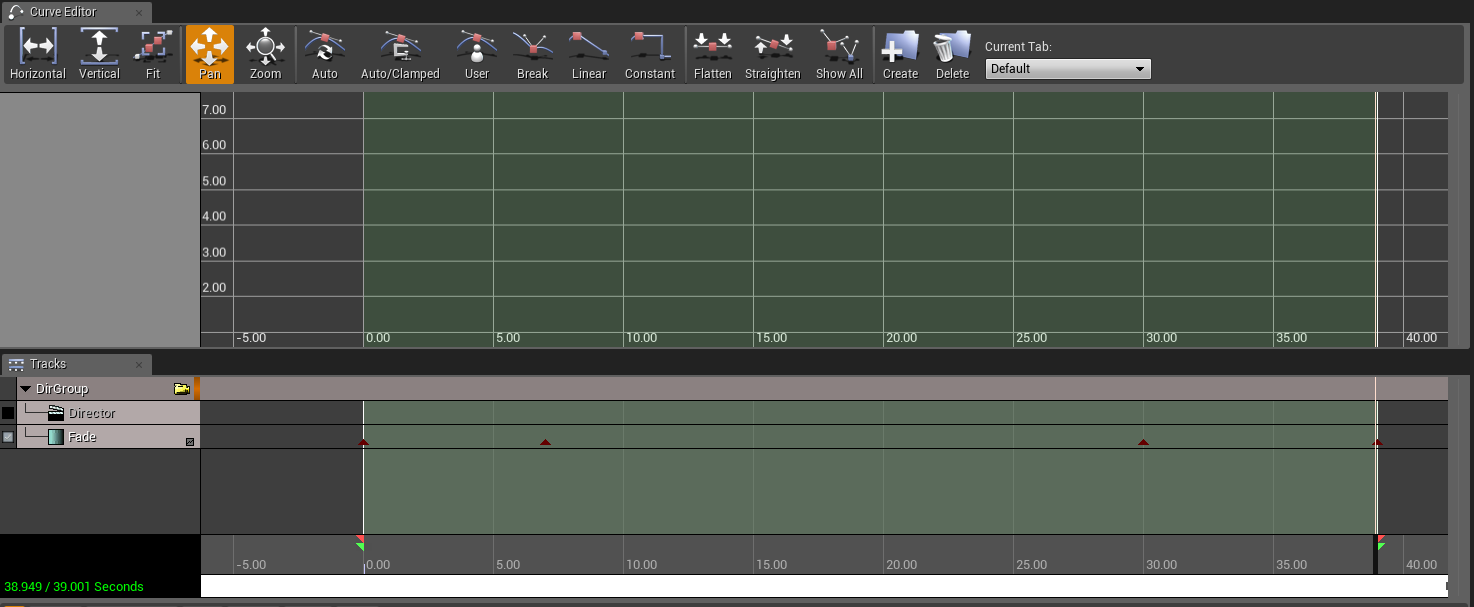
\includegraphics[width=\textwidth]{Images/matinee.png} 
\caption[Konfiguration der Matinee]{Konfiguration der Matinee; rote Dreiecke = Keys; gr{\"u}ner Bereich = Anzeigedauer.}
\label{fig-matinee} 
\end{figure}


Somit ist das erste Bild f{\"u}r das Szenario fertig konfiguriert. 
Dieser Ablauf wurde f{\"u}r acht weitere Bilder durchgef{\"u}hrt. \\

Der Wechsel zwischen den Bildern f{\"u}r das Hauptszenario wurde anhand der Level-Option von Unreal vorgenommen. 
Diese Option besteht aus einem anhaltenden Level und beliebig viele Level, die hinzugef{\"u}gt werden k{\"o}nnen. 
In diesem Fall acht Level f{\"u}r die verwendeten Bilder. 
Das anhaltende Level beinhaltet die Audio-Datei und verwaltet den Wechsel der Bilder, welches alle 39 Sekunden durchgef{\"u}hrt wird. Die 39 Sekunden kamen zustande, in dem die L{\"a}nge der Audio-Datei durch die Anzahl der Bilder geteilt wurde. 
Damit wurde vermieden das die Audio-Datei von Anfang an abgespielt wird. 
Ein gro{\ss}er Vorteil der Level-Option ist, dass die Audio-Datei fortl{\"a}uft, auch w{\"a}hrend dem Level-Wechsel und somit keine Unterbrechungen entstehen. 
Da das WarmUp f{\"u}r das Gl{\"u}cks-Szenario nur aus einem Bild besteht, musste hier keine Level-Option konfiguriert werden. \\

